% Copyright © 2013 Martin Ueding <dev@martin-ueding.de>

\input{header.tex}

\usepackage{tikz}
\usetikzlibrary{calc}

\hypersetup{
	pdftitle=
}

\title{Skizze zur Pyramide}
\author{
	Martin Ueding \footnote{\href{mailto:mu@martin-ueding.de}{mu@martin-ueding.de}}
}

\begin{document}

\maketitle

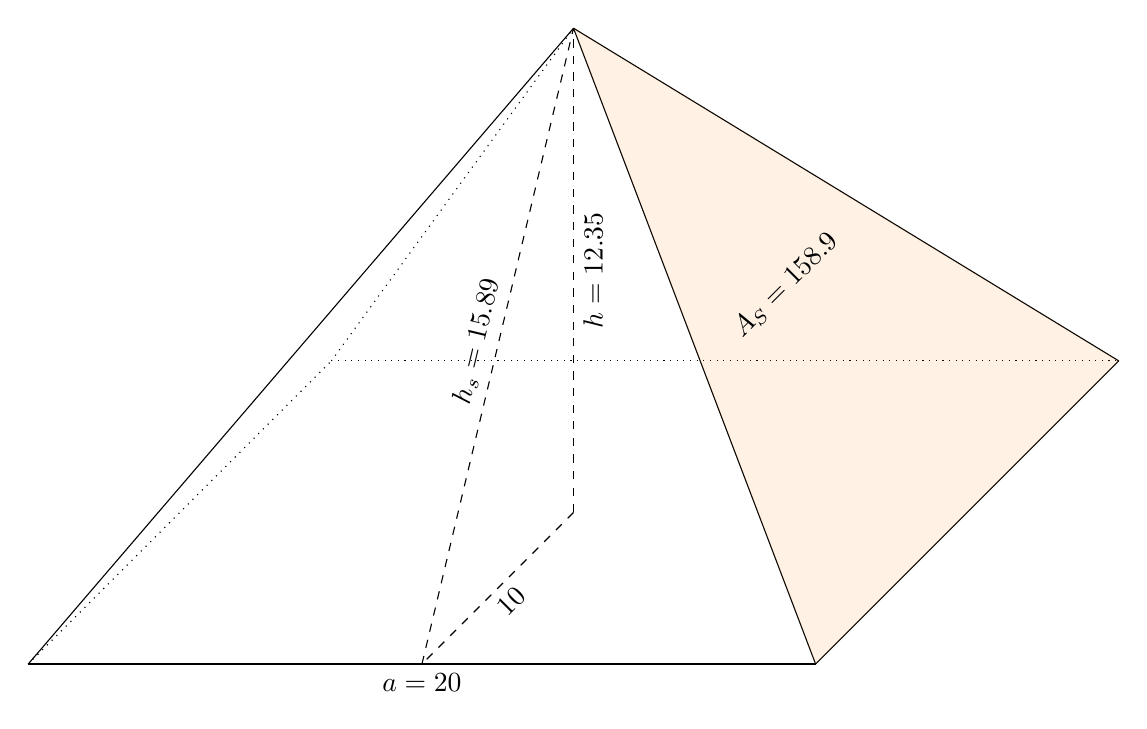
\begin{tikzpicture}[scale=50]
	\draw[dotted] (0, 0, 0) -- (.2, 0, 0);
	\draw (.2, 0, 0) -- (.2, 0, .2);
	\draw (.2, 0, .2) -- (0, 0, .2) node[midway, below, sloped] {$a = \SI{20}{\centi\meter}$};
	\draw[dotted] (0, 0, .2) -- (0, 0, 0);
	\draw[dotted] (0, 0, 0) -- (.1, .123, .1);
	\draw (.2, 0, 0) -- (.1, .123, .1);
	\draw (.2, 0, .2) -- (.1, .123, .1);
	\draw (0, 0, .2) -- (.1, .123, .1);
	\draw[dashed] (.1, 0, .2) -- (.1, .123, .1) node[midway, sloped, above] {$h_s = \SI{15.89}{\centi\meter}$};
	\draw[dashed] (.1, 0, .1) -- (.1, .123, .1) node[midway, sloped, below] {$h = \SI{12.35}{\centi\meter}$};
	\draw[dashed] (.1, 0, .1) -- (.1, 0, .2) node[midway, sloped, below] {$\SI{10}{\centi\meter}$};

	\fill[opacity=.10, color=orange] (.2, 0, 0) -- (.1, .123, .1) -- (.2, 0, .2);
	\path ($(.2, 0, 0)!.5!(.1, .123, .1)$) -- ($(.2, 0, .2)!.5!(.1, .123, .1)$) node[below, midway, sloped] {$A_S = \SI{158.9}{\centi\meter\squared}$};
\end{tikzpicture}

%\newpage
%\tableofcontents
%\newpage

%\IfFileExists{\bibliographyfile}{
%	\bibliography{\bibliographyfile}
%}{}

\end{document}

% vim: spell spelllang=de
